\clearpage
\section{Monopol (charakteristiky, typy monopolů, rovnováha monopolu, chování monopolu
oproti dokonalé konkurenci, efektivnost monopolu a cenová diskriminace, regulace
monopolu).}

\subsection{Charakteristiky}
Je to taková tržní situace, kdy na trh daného produktu dodává jediná firma. Tato
firma není vystavena konkurenci jiných firem, které by dodávaly stejný či podobný produkt.

\subsection{Typy monopolů}
\begin{enumerate}
    \item \textbf{Administrativní monopol} - Je-li vstup na trh vázán na povolení státu a dá-li stát 
    toto povolení pouze jediné firmě, získá tato firma administrativní monopol.
    \item \textbf{Přirozený monopol} - Přirozený monopol vzniká z důvodu přirozených bariér vstupu na trh.
    Tato situace nastává, když jsou dodávky zboží či služby vázány na určitou přenosovou síť. 
    stup na trh druhé firmě sice nikdo nezakazuje, ale brání jí v něm vysoké náklady, které by 
    musela vynaložit na vybudování vlastní přenosové soustavy, bez níž není možné zboží či služby dodávat.
\end{enumerate}

\subsection{Rovnováha monopolu}
Představuje takový objem produkce, při kterém firma maximalizuje zisk, přičemž musí být splněna
obecná podmínka MR = MC. Tento objem výroby je však menší než u dokonale konkurenční firmy 
za jinak stejných podmínek. Monopolní zisk je pak dán úsečkou $m$ v grafu níže, dosahuje ekonomického zisku.
Křivka nabídky v monopolu neexistuje, nabídka je fixní.

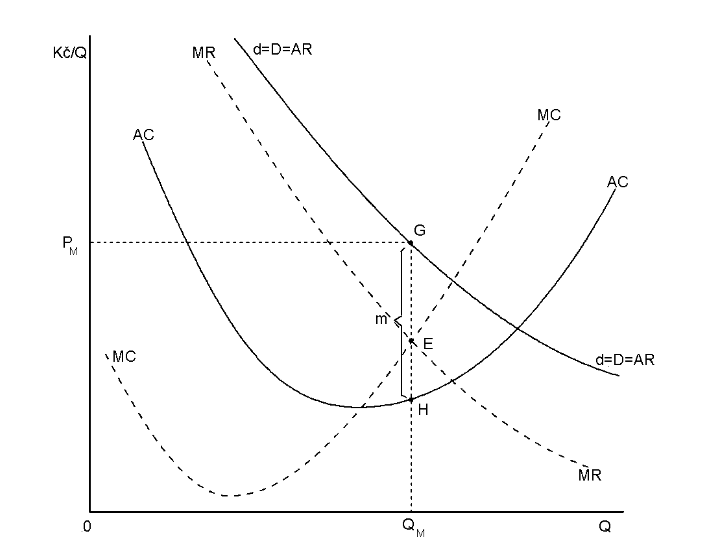
\includegraphics[width=16cm]{images/13_rovnovaha.png}

\subsection{Chování monopolu oproti dokonalé konkurenci}
Monopol nabízí menší množství a za vyšší cenu. Dosahuje ekonomického zisku, který nazýváme
monopolním ziskem. Platí-li spotřebitelé vyšší cenu, dochází k přerozdělování zisku na úkor 
spotřebitelů a ve prospěch monopolu. Monopol tedy vyvolává neefektivnost - poskytuje menší 
než optimální množství. Monopol tak způsobuje celospolečenské ztráty, tzv. společenské náklady monopolu.

\subsection{Efektivnost monopolu}
Efektivnost firem posoudíme, když porovnáme mezní náklady s mezním užitkem. Monopol
maximalizuje svůj zisk při takovém objemu výroby, při kterém se mezní příjem rovná
mezním nákladům (MR = MC). Objem výroby v odvětví s monopolem maximalizujícím zisk je tedy
nižší než objem výroby optimální pro společnost. Lze říci, že nedokonale konkurenční trhy jsou méně
efektivní než dokonale konkurenční trhy.\\
Skutečnost, že monopol disponuje určitou monopolní silou, mu umožňuje používat v cenové
strategii tzv. \textbf{cenovou diskriminaci}. Podstatou cenové diskriminace je stanovení rozdílných
cen stejných výrobků, aniž by k tomu vedly nákladové důvody (slevy pro studenty, děti, důchodce).

\subsection{Regulace monopolu}
\begin{enumerate}
    \item \textbf{Antitrustové zákonodárství} - omezují monopolizaci ekonomiky tím, že zakazují určité
    konkrétní chování firem (například jejich spojování, dohody o cenách apod.) - Úřad na
    ochranu hospodářské soutěže.
    \item \textbf{Ekonomická regulace} - pravidla nebo zákony, kterými stát ovlivňuje nebo
    kontroluje činnost firem. Ekonomická regulace se liší od cenové regulace tím, že neurčuje
    konkrétní ceny konkrétních výrobků, ale spíše stanoví pravidla pro cenovou tvorbu.
    \item \textbf{Daňová politika} - zvýšení daní sice snižuje zisky monopolů, ale neprojevuje se přímo
    ve velikosti vyráběného objemu produkce.
    \item \textbf{Převedení monopolu} do státního vlastnictví - je nástrojem, jehož použití ve větší míře než
    nástroje dosud zmíněné determinují širší okolnosti (politický systém, kultura, historie,
    tradice apod.).
    \item \textbf{Cenová regulace} - představují centralizované stanovení ceny konkrétních statků.
\end{enumerate}